\documentclass{paper}

%\usepackage{times}
\usepackage{epsfig}
\usepackage{graphicx}
\usepackage{amsmath}
\usepackage{amssymb}
\usepackage{color}
\usepackage{caption}
\usepackage{subcaption}


% load package with ``framed'' and ``numbered'' option.
%\usepackage[framed,numbered,autolinebreaks,useliterate]{mcode}

% something NOT relevant to the usage of the package.
\setlength{\parindent}{0pt}
\setlength{\parskip}{18pt}
\graphicspath{{images/}}


\usepackage[latin1]{inputenc} 
\usepackage[T1]{fontenc} 


\usepackage{listings} 
\lstset{% 
   language=Matlab, 
   basicstyle=\small\ttfamily, 
} 



\title{Assignment 3}



\author{Jenni Simon\\09-116-005}
% //////////////////////////////////////////////////


\begin{document}



\maketitle


% Add figures:
%\begin{figure}[t]
%%\begin{center}
%\quad\quad   \includegraphics[width=1\linewidth]{ass2}
%%\end{center}
%
%\label{fig:performance}
%\end{figure}

\section*{Video search with bags of visual words}


\paragraph{1. Data aquisition}

The video data used during this assignment stems from an episode of the TV series 'Arrested Development'. SIFT descriptors computed using VLFEAT (http://www.vlfeat.org) are used as local feature descriptors. The video sequence consists of 918 frames and a total of 810'650 SIFT descriptors have been computed from them.

\begin{figure*}[h!]
    \centering
    \begin{subfigure}[]{0.5\textwidth}
        \centering
        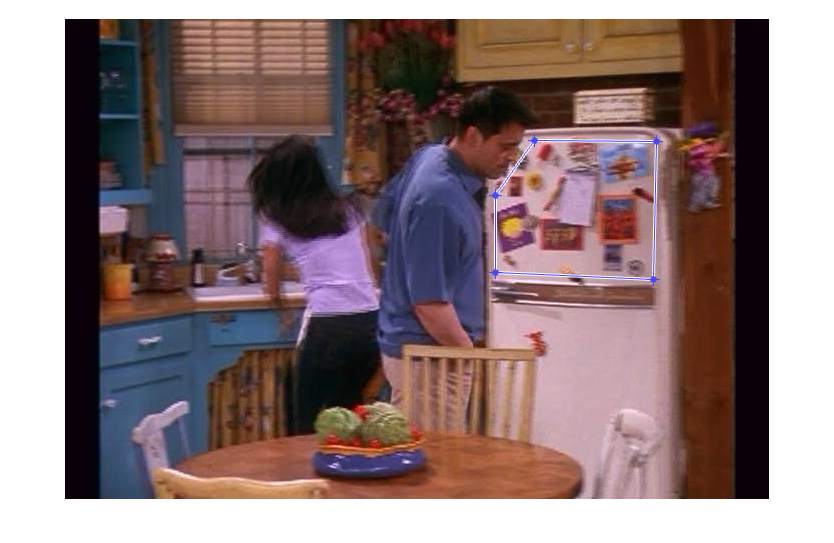
\includegraphics[width=\textwidth]{rawMatchSel.png}
    \end{subfigure}%
    ~ 
    \begin{subfigure}[]{0.5\textwidth}
        \centering
        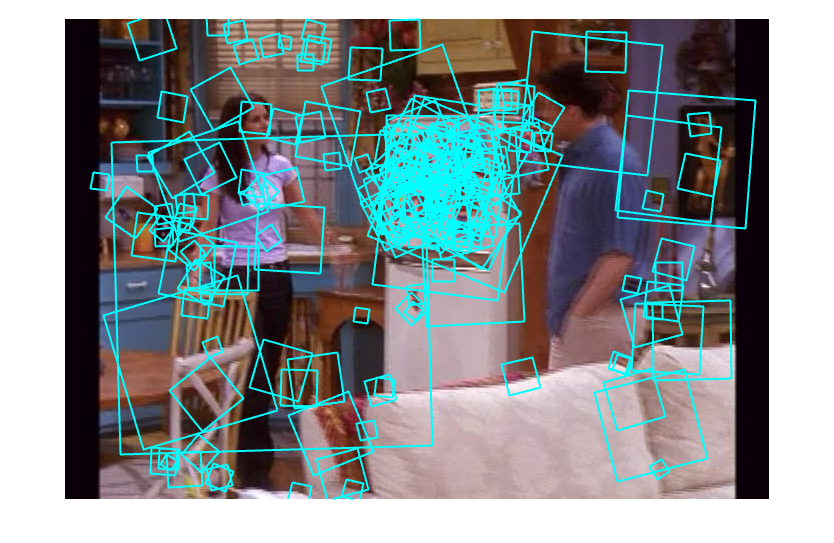
\includegraphics[width=\textwidth]{rawMatchRes.png}
    \end{subfigure}
    \caption{The result of matching the raw SIFT-descriptors in the selected region of the left image with the SIFT-descriptors of the right image.}
\label{fig:rawMatch}
\end{figure*}

\paragraph{2. Raw descriptor matching}
The goal of this part of the assignment was to let the user select a region in one of two provided images, compute the SIFT-descriptors located inside this region and finally computing and displaying the best matching sift descriptors in the second image for each descriptor in the selected region. The matching of the descriptors has been done by simply computing the nearest neighbours (in $l^2$-norm) of the region-descriptors to the descriptors of the second frame. An example result is shown in figure \ref{fig:rawMatch}.

\paragraph{3. Computing and visualising the vocabulary}
The objective of this part is to quantise the computed descriptors into clusters. These clusters can be viewed as words of  a visual vocabulary the images are consisting of. The images in this context can be viewed as documents (containing words). 

The cluster centres are computed using $K$-Means. As we are dealing with a relatively big amount of data, only the descriptors of a subset of the frames has been used in the computation of the centres. Concretely, only every $k^{th}$ frame of the video is used and a ratio of $p$ descriptors of the frame are used for the computation of the clusters. Choosing every $k^{th}$ frame instead of just choosing $N/k$ frames ($N:=$ number of frames) uniformly random has the advantage that each scene is guaranteed to be represented by some frames and seemed to give better results. The number of cluster-centres  was chosen as $K=1600$, the ratio of descriptors per frame was chosen as $p=0.9$ and $k=10$. Figure \ref{fig:vocab} shows some image-patches corresponding to two of the resulting visual words.

\begin{figure*}[h!]
    \centering
    \begin{subfigure}[]{0.5\textwidth}
        \centering
        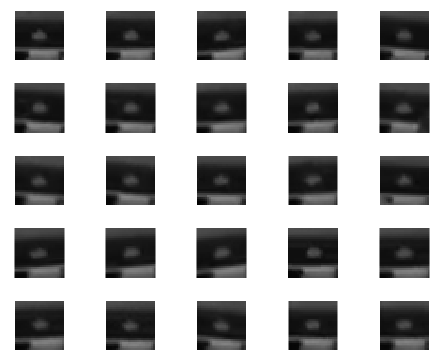
\includegraphics[width=0.9\textwidth]{examplesWord1.png}
    \end{subfigure}%
    ~ 
    \begin{subfigure}[]{0.5\textwidth}
        \centering
        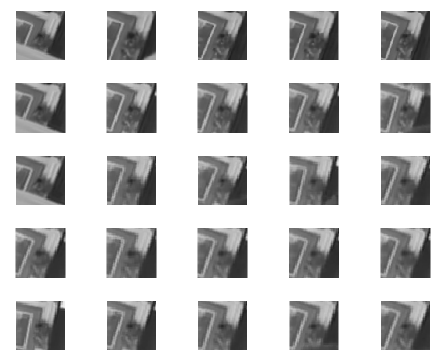
\includegraphics[width=0.9\textwidth]{examplesWord3.png}
    \end{subfigure}
    \caption{25 example patches corresponding to two visual words.}
\label{fig:vocab}
\end{figure*}

The two words shown in figure \ref{fig:vocab} have been chosen as very distinct (high distance in feature-space) and we can clearly observe them describing two distinct image features.


\paragraph{4. Full frame queries}
Now that we have computed the vocabulary we can use it to query the frames of the video. In this part of the assignment we use it to query the video for frames most similar to a given query frame. To this end, we pre-compute the  bag-of-words histograms for each of the frames in the video. That is, for each frame $f$ we map each descriptor $d$ to the closest word and accumulate the number of descriptors per word in a vector $v_f=(t_{f1},...,t_{fK})$ where $K$ is the number of words and $t_{fi}$ is the number of occurrences of word $i$ in frame $f$. We can then compute the matching score between a query frame $q$ and a frame $f$ by computing the normalised scalar-product between the vectors $v_f$ and $v_q$, that is we define:
\begin{equation}
score(q,f)= \frac{v_q\cdot v_f}{|v_q| | v_f|}
\end{equation}
By assigning to each query $q$ an array of scores $S(q)=[score(q,1),...,score(q,K)]$ and sorting it, we can retrieve the $m$ best matches for the query $q$. Figures \ref{fig:fullfFame1} and \ref{fig:fullfFame2} show query frames and the five best matches found by the described method.

We observe that the method in general works very well at retrieving similar frames from the dataset. Only the last example in figure \ref{fig:fullfFame2} shows some result with a  significantly different frame (still belonging to the same scene but from an opposite viewpoint). 

\begin{figure*}[h!]
    \centering
    \begin{subfigure}[]{\textwidth}
        \centering
        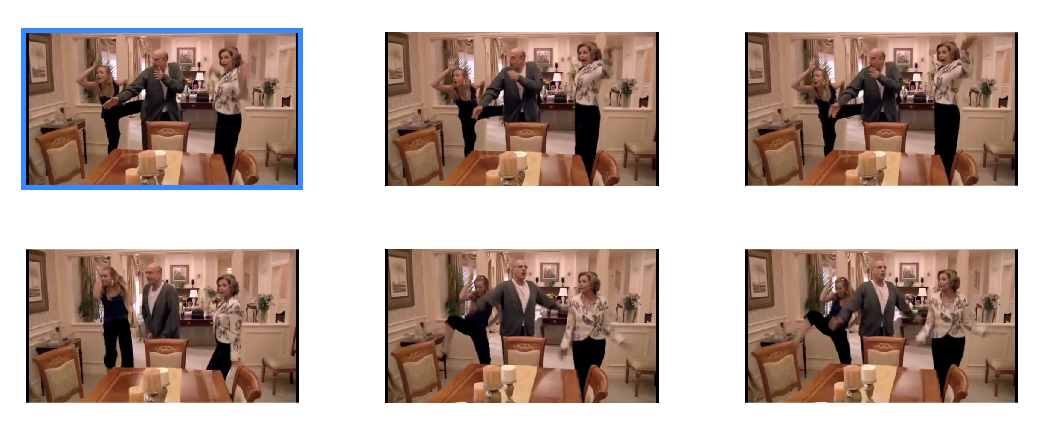
\includegraphics[width=\textwidth]{query1.png}
    \end{subfigure}
    \begin{subfigure}[]{\textwidth}
        \centering
        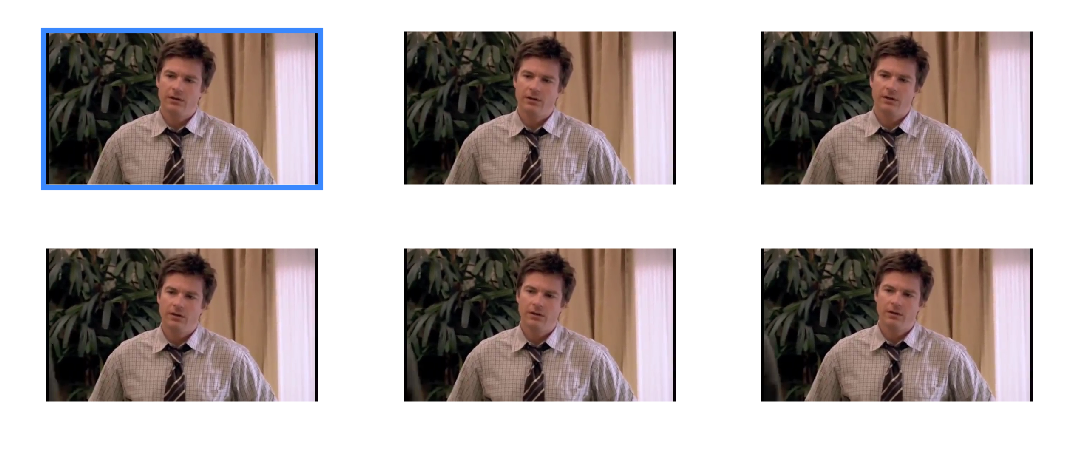
\includegraphics[width=\textwidth]{query6.png}
    \end{subfigure}
        \caption{Results of full frame queries. The upper left image (blue frame) is the query frame followed by the five best matching frames. }
\label{fig:fullfFame1}
\end{figure*}

\begin{figure*}[h!]
    \centering
    \begin{subfigure}[]{\textwidth}
        \centering
        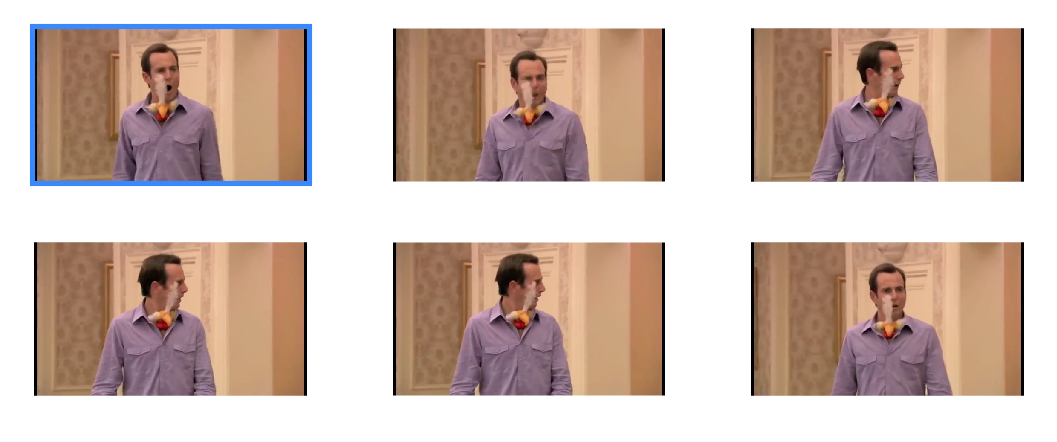
\includegraphics[width=\textwidth]{query3.png}
    \end{subfigure}
    \begin{subfigure}[]{\textwidth}
        \centering
        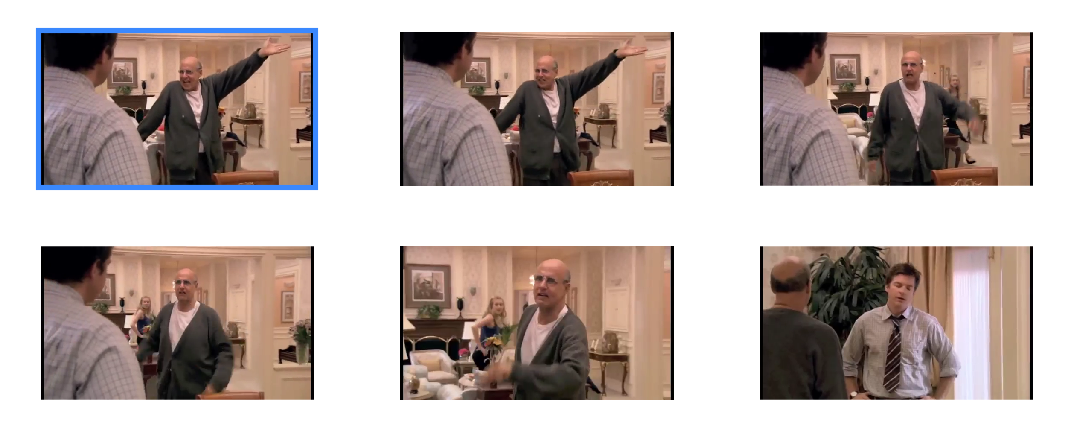
\includegraphics[width=\textwidth]{query5.png}
    \end{subfigure}
    \caption{Results of full frame queries. The upper left image (blue frame) is the query frame followed by the five best matching frames. }
\label{fig:fullfFame2}
\end{figure*}


\paragraph{5. Region queries}
Rather than querying a whole frame we might be more interested in querying for a region of the image. In order to adjust the system for this task we draw inspiration from text retrieval methods by employing a standard weighting scheme called 'term frequency-inverse document frequency' or short $tf$-$idf$. We therefore represent each frame with a new weighting vector $\tilde{v}_f=(v_{f1},...,v_{fK})$ where $v_{fi}$ is given by:
\begin{equation}
\tilde{v}_{fi}= \frac{t_{fi}}{n_f}\text{log} \frac{N}{m_i}
\end{equation}
Here, $t_{fi}$ is again defined as the number of occurrences of visual-word $i$ in frame $f$, $n_f$ is the number of words in frame $f$, $N$ is the number of frames and $m_i$ the number of frames containing word $i$. The intuition behind these weights is that the term-frequency $\frac{t_{fi}}{n_f}$ indicates the relative importance of each word to the frame (high weight to words occurring often in frame) and the inverse-document-frequency $\frac{N}{m_i}$ indicates how "common" word $i$ is among all the frames (high weight to words occurring seldom among all frames).

Words that occur in almost all frames convey not much information to which frame best matches our query and can in fact introduce many mis-matches. To mitigate this issue the top 3\% of the most common words (stop words) are dropped from the vocabulary altogether. 

Let $v_q=(t_{q1},...,t_{qK})$ be the vector consisting of the number of occurrences of all the words in the query region. The matching score is then given by:
\begin{equation}
score(q,f)= \frac{v_q\cdot \tilde{v}_f}{|v_q| | \tilde{v}_f|}
\end{equation}
The same method as in the previous paragraph can be applied to find the $m$ best matching frames for the region. Figures \ref{fig:regMatch1} and \ref{fig:regMatch2} show some example results. 

\begin{figure*}[h!]
    \centering
    \begin{subfigure}[]{\textwidth}
        \centering
        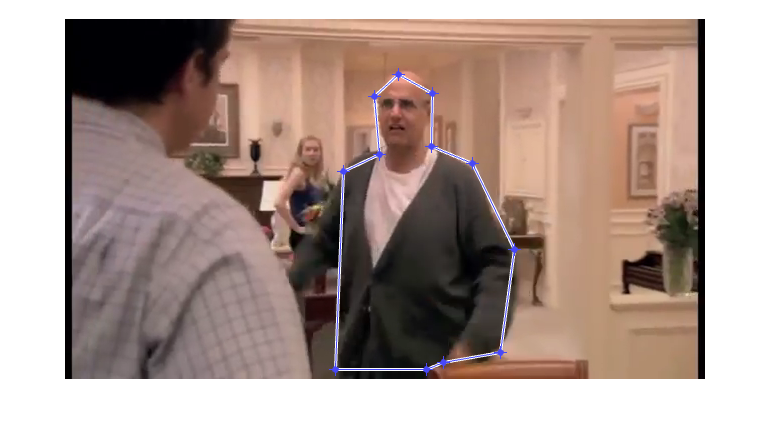
\includegraphics[width=0.6\textwidth]{regionQuery1sel.png}
    \end{subfigure}
    \begin{subfigure}[]{\textwidth}
        \centering
        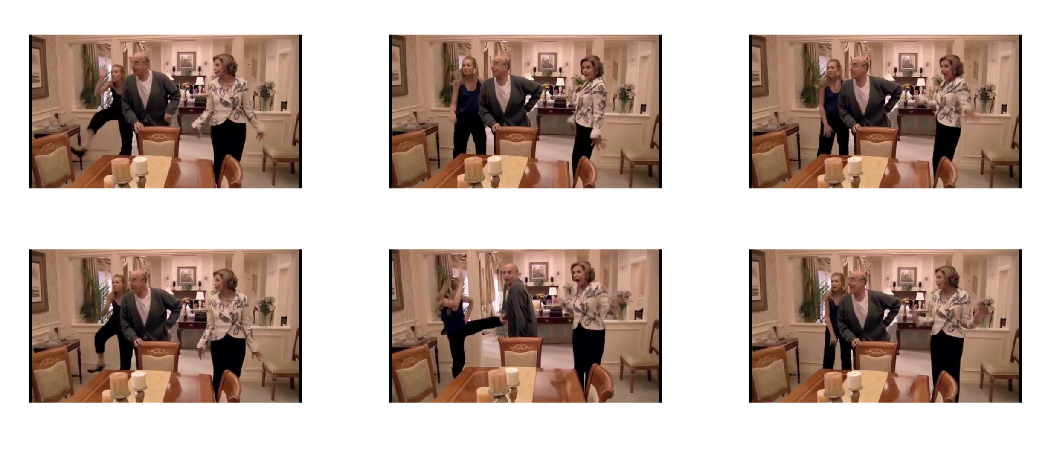
\includegraphics[width=\textwidth]{regionQuery1res.png}
    \end{subfigure}
    \begin{subfigure}[]{\textwidth}
        \centering
        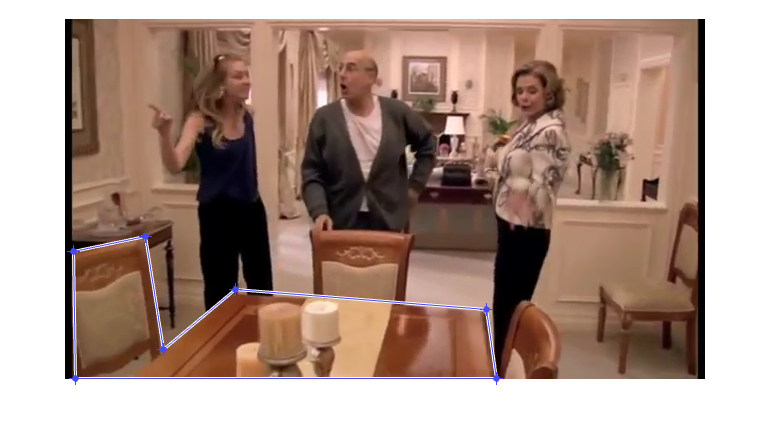
\includegraphics[width=0.6\textwidth]{regionQuery2sel.png}
    \end{subfigure}
    \begin{subfigure}[]{\textwidth}
        \centering
        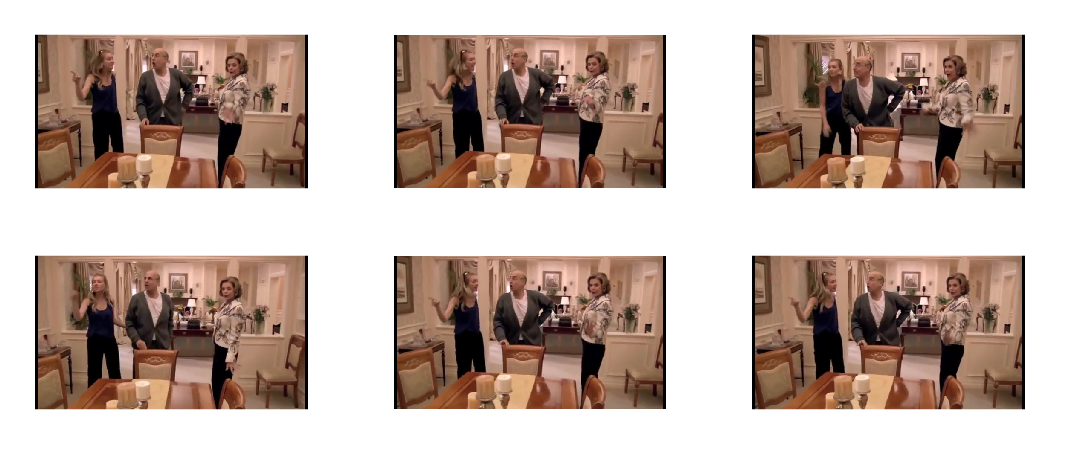
\includegraphics[width=\textwidth]{regionQuery2res.png}
    \end{subfigure}
    \caption{Results of region queries. The upper image is the frame with the selected query region, followed by the six best matching frames. }
\label{fig:regMatch1}
\end{figure*}

We observe that when querying relatively big regions as in figure \ref{fig:regMatch1}, the method works very well at retrieving similar frames. However, when querying smaller regions as in figure \ref{fig:regMatch2}, the results are less convincing at first glance. In the upper query of figure \ref{fig:regMatch2}, there is in fact no frame retrieved showing the exact plant that has been queried. One reason for this miss-matching can be found when looking at the number of words in the query-region. The plant region with around 22 words shows by far the lowest word-count. The flower, with around 55 words, has the second lowest count and indeed the flower is actually visible in all the retrieved frames (in the background at smaller scale). The more words per query, the more accurate the results when comparing the region-statistics to the full-frame statistics.

\begin{figure*}[h!]
    \centering
    \begin{subfigure}[]{\textwidth}
        \centering
        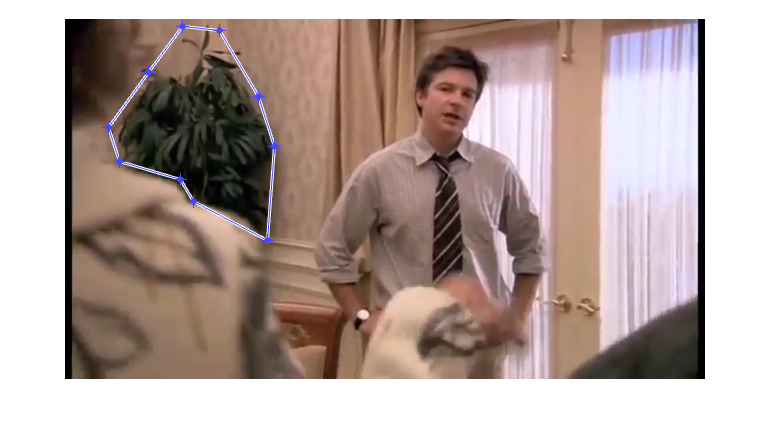
\includegraphics[width=0.6\textwidth]{regionQuery3sel.png}
    \end{subfigure}
    \begin{subfigure}[]{\textwidth}
        \centering
        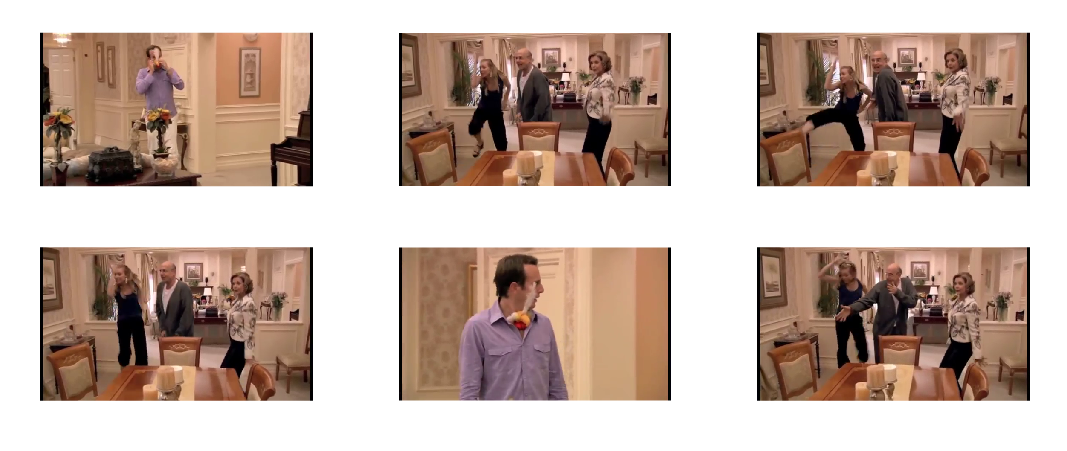
\includegraphics[width=\textwidth]{regionQuery3res.png}
    \end{subfigure}
    \begin{subfigure}[]{\textwidth}
        \centering
        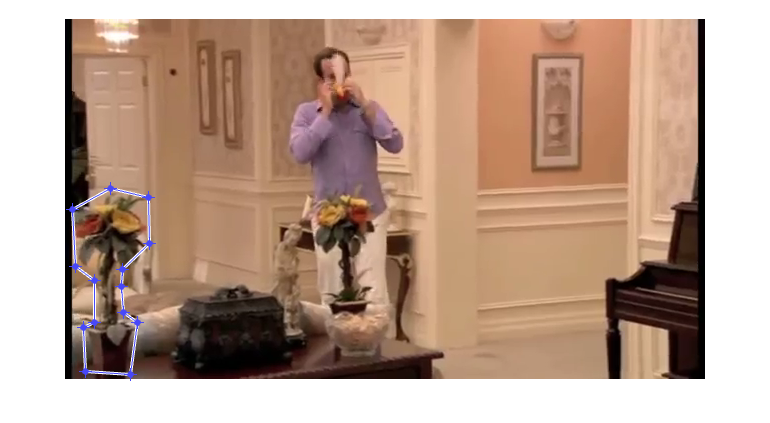
\includegraphics[width=0.6\textwidth]{regionQuery4sel.png}
    \end{subfigure}
    \begin{subfigure}[]{\textwidth}
        \centering
        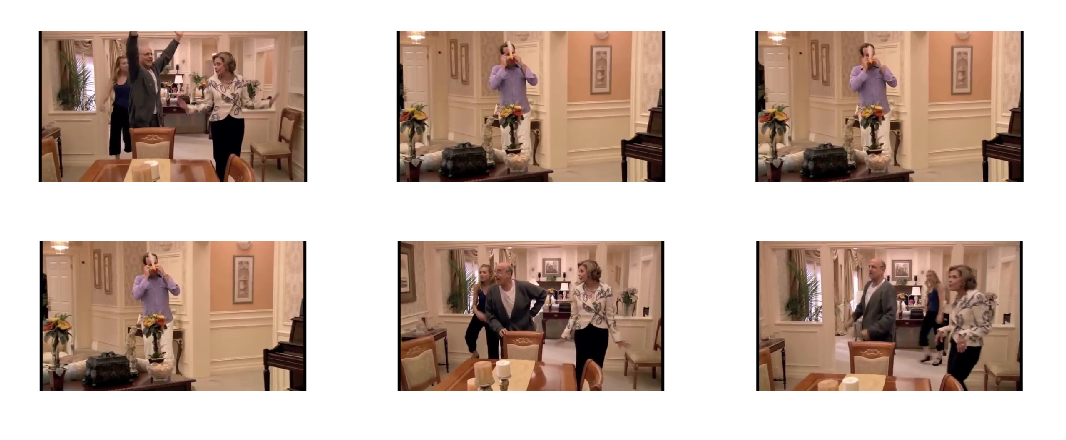
\includegraphics[width=\textwidth]{regionQuery4res.png}
    \end{subfigure}
    \caption{Results of region queries. The upper image is the frame with the selected query region, followed by the six best matching frames. }
\label{fig:regMatch2}
\end{figure*}



%\begin{figure*}[h!]
%    \centering
%    \begin{subfigure}[]{0.33\textwidth}
%        \centering
%        \includegraphics[height=1.2in]{}
%    \end{subfigure}%
%    ~ 
%    \begin{subfigure}[]{0.33\textwidth}
%        \centering
%        \includegraphics[height=1.2in]{}
%    \end{subfigure}
%    \caption{Recovered gray albedo}    
%\label{fig:GA}
%\end{figure*}

 \end{document}